% ============================= Info ============================= %

% Applied Machine Learning Systems ELEC0132 Assignment
% Due 11:59pm, 07 Jan 2019

% 6 double-column single-spaced pages 
% Plus up to 4 pages of supplementary material 
% (methodology clarification, additional results, other tests, etc.)

% Include hidden link to code in public repo (Dropbox, Drive, etc.)

\iffalse
Assignment tasks:
	- Detection and removal of noisy images
	- Training, validation and testing subsets division
	- Train ML models to perform
		Binary tasks
			1. Emotion recognition (smile/!smile)
			2. Age identification (young/old)
			3. Glasses detection (with/without)
			4. Human detection (real/avatar)
		Multiclass tasks
			5. Hair colour recognition (ginger, blond, brown, grey, black, bald)
\fi

% =========================== Packages =========================== %
\documentclass[conference]{IEEEtran}
\usepackage{amsmath, graphicx, multicol, cite}
\usepackage{color}
\usepackage{listings}% code
%\usepackage{refcheck}
\usepackage[colorlinks = true,
            linkcolor = black,
            urlcolor  = blue,
            citecolor = black,
            anchorcolor = blue]{hyperref}

\lstset{escapeinside={<@}{@>}}

% ============================= Title ============================= %
\begin{document}
\def\code#1{\texttt{#1}}

\title{Applied Machine Learning\\
 Systems ELEC0132 Assignment}
\author{\large Maryam Habibollahi\\ \textit{Department of Electronic and Electrical Engineering}\\ \textit{University College London}\\ zceemha@ucl.ac.uk}
\date{November 2018}
\maketitle

\setcounter{page}{1} \pagenumbering{arabic}

% ============================ Abstract =========================== %
\begin{center} \large \textbf{Abstract} \end{center}
% \textit{Brief overview of the methodology/results presented.}\\

Machine learning algorithms have been implemented for the detection and classification of human faces with binary and multiclass attributes using the Python programming language with several image manipulation and machine learning libraries. A comparative analysis of the performance of the different techniques for face detection and classification provided a higher obtainable accuracy from neural network architectures, particularly the single-shot-multibox detector for accurate face detection, the multi-layer perceptron model for binary classification tasks, with accuracies above 0.8, and the LeNet convolutional neural network architecture for multiclass classification, providing an accuracy of 0.81 on the hair colour classification task. The code and all results can be accessed via  \href{https://drive.google.com/file/d/1WXVxgsFRLl0BnZnKn3MUFrzJA3oxCLS6/view?usp=sharing}{Google Drive} or directly from the  \href{https://github.com/maryamhb/AMLSassignment}{GitHub repository}.

% ========================== Introduction ========================== %
\section{Introduction} \label{s-intro}

% The problem statement.\\

% Why face recognition, why classification? (applications, need, PROBLEM!)
The perception of visual information is a key element of human communication, particularly those from the face. The features and characteristics of an individual's face can provide information about their identity, emotion, and intent, with potential applications in access and security, law enforcement, marketing, and banking. Researchers in the fields of computer vision have been developing technological breakthroughs %?
in the implementation of face recognition using machine learning tools and techniques over the past decades.
% Problem
The variations in real-world images from illumination, pose, expressions, and occlusions have required more complex learning tools to provide adequate predictions for a variety of images. A suitable balance between a model's accuracy and complexity is often required to meet the computational power limitations and performance requirements of a system.

% Assignment + dataset description:
% summarising data (content, size, format, etc.) and describing any \textit{data preprocessing} applied.\\

This assignment aims to train machine learning models and perform binary and multiclass classification on a large dataset of 5000 Portable Network Graphic (PNG) image files consisting of pre-processed subsets from the "CelebFaces Attributes Dataset (CelebA)", a celebrity image dataset \cite{Yang2015} , and the "Cartoon Set", an image dataset of random cartoons/avatars \cite{Cole}, as well as a number of noisy images (mainly of natural backgrounds) to be detected and removed from the training data, containing 80\% of the entire dataset.
All images include five labels; a multiclass hair colour label, and four binary labels classifying human/non-human subjects, whether the subject is young, wearing glasses, and smiling.

In order to train a suitable model for the required classification tasks, several preprocessing methods were taken into consideration to provide appropriate features for the process; for instance, facial landmarks were extracted upon face detection to train models using supervised learning algorithms such as Support Vector Machines (SVM) or  Multi-Layer Perceptron (MLP) models based on the extracted facial landmarks.
A comparative analysis of the performance of each method with respect to the labelled noisy images facilitated the selection of the most appropriate feature extraction method for the given dataset.

Prior to the extraction of features, various preprocessing techniques were carried out on the images to improve both the performance and processing power during the later stages of the extraction, training and classification procedures. 
Examples of such techniques include colour space transformation, capable of significantly reducing processing complexity, gamma correction (power-law equalisation), a non-linear function used to normalise illumination by raising the input value to the power $\gamma$, as shown in Equation \ref{eq: gamma}, and mean normalisation.

\begin{equation}
V_{out} = AV_{in}^{\gamma} \hspace{0.2cm} \text{, where  A = 1 in the common case}
\label{eq: gamma}
\end{equation}


The original dataset was otherwise rescaled and augmented to avoid overfitting for alternative models more specifically used for visual recognition tasks, such as Convolutional Neural Networks (CNN), where the noisy images of the training and validation data are removed using the results of the optimum face detector method with the maximum accuracy. % Duh

% ======================= Proposed algorithms ====================== %
\section{Proposed algorithms} \label{s-algorithms}

% Algorithmic approach used to solve the problem.\\
% Explain rationale behind choices, i.e. detail your \textit{reasons for selecting a particular model}.\\

% Feature extraction methods 
A major step of the extraction of facial information for various classification tasks such as age, gender, emotion, and other attributes apparent on the face is to localise the fiducial facial key points \cite{landmark_lit}. The landmarks provide a set of $x$ and $y$ coordinates that either describe the specific points that describe a unique location of a particular component, or lay out the contours connecting those points, such as those shown in Figure \ref{fig: landmarks}.
Several algorithms have been developed to achieve this purpose, namely the Haar cascade classifier, the first real-time face detector proposed in 2001, the Histogram of Oriented Gradients feature with a linear classifier, and various Deep Learning-based detectors, which are significantly more accurate than the former two methods, though at a cost of higher complexity.
% TODO: How does the HOG work?

\begin{figure} [h] % Landmarks
  \centering
    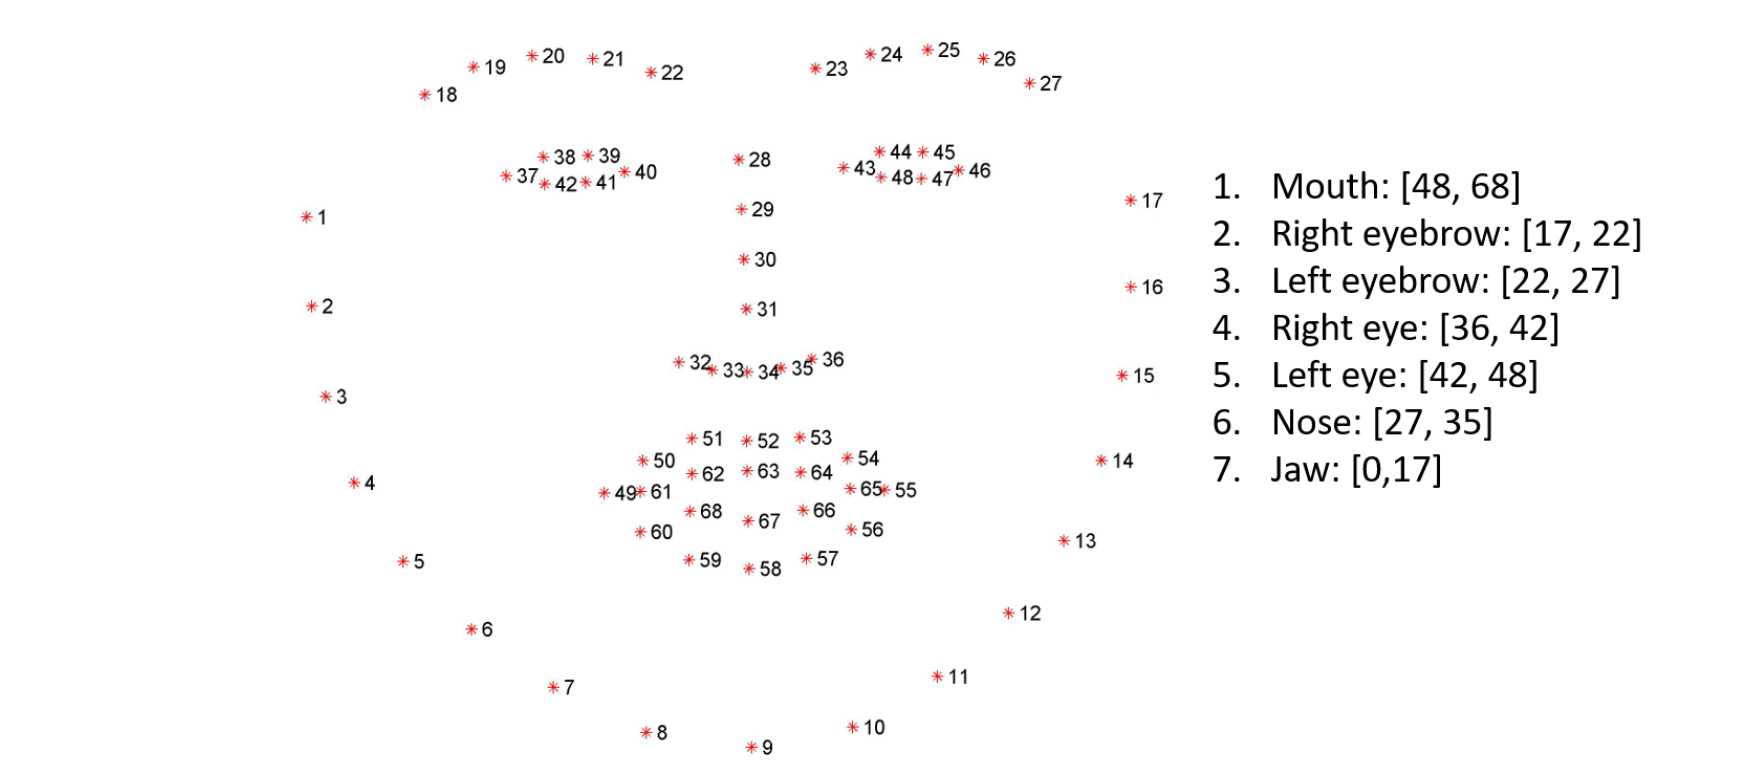
\includegraphics[width=0.5\textwidth]{graphs/landmarks} 
    \caption{Face shape defined by 68 landmarks}
    \label{fig: landmarks}
\end{figure}

% Deep learning-based
One such Deep Learning-based face detector based on Deep Neural Networks (DNN) is known as the Single-Shot-Multibox Detector (SSD), which uses the ResNet-10 architecture as a backbone. This method is ideal for a dataset with various orientations and considerable occlusion in the images; however, the complexity of the model requires a longer amount of time to carry out the detection.
Another detector with Convolutional Neural Network (CNN) features is called the Maximum-Margin Object Detector (MMOD), which has a simple training process; though also more complex than the former two detectors.
% HOG is better
The relative balance between the expected accuracy and complexity of a HOG detector with respect to the Haar cascade and Deep Learning options makes it preferable for this dataset. Nonetheless, a comparative analysis was performed by recording the accuracy and training time of each detector as a measure of performance and complexity.

% SVM model
Classification of the binary tasks was performed using the landmark features to train models with supervised learning algorithms, namely Support-Vector Machines (SVM), which are capable of linearly separating classes in a high-dimensional space through the implementation of different kernel functions. 
% Gradient descent
The hyperplane which isolates one class from another can be refined via gradient descent, an iterative optimisation algorithm, such as that shown in Equation \ref{eq: GD}, which represents the gradient in linear regression for a model of n data points and m features. This technique is used to minimise a parameter called the cost function, which represents an attribute of the error in the response, such as the squared sum of residuals.
% TODO: Hyperparameter selection

\begin{equation}
\theta_{j+1} = \theta_j - \frac{\alpha}{n} \sum_{i=1}^n \bigg[\sum_{k=1}^m \theta_k x_k^{(i)} - y^{(i)} \bigg] x_j^{(i)} 
\label{eq: GD}
\end{equation}

% MLP model
Higher-complexity models based on artificial neural networks that are capable of providing higher accuracies were also implemented using the features extracted. A Multi-Layer Perceptron (MLP) model, which carries out the training using Backpropagation, an efficient method that computes the partial derivates in gradient descent, was therefore selected for the binary tasks. The derivatives are calculated from each layer's error term, $\delta_i^l$, which is computed using Equation \ref{eq: backprop}, for $a^{(l)}$ representing the activation vector of layer $l$, resulting in the output $z^{(l)} = \theta^{(l)} a^{(l)}$ for that layer.
% TODO: Hyperparameter selection

\begin{equation}
\delta^{(l)} = \big(\theta^{(l)}\big)^T \delta^{(l+1)}.g'(z^{(l)})
\label{eq: backprop}
\end{equation}

% CNN model
Despite the minimised processing requirement when the landmark features are used, they pose limitations to classification tasks less reliant on the key component locations, and requiring important information omitted from the images such as colour. Thus, for the final task of detecting hair colour, a more commonly-used classifier for image processing with multilayer neural networks called Convolutional Neural Networks (CNN) was implemented on a LeNet architecture. The popularity of CNNs in image classification is primarily due to the 3D volumes of neurons, resulting in connectivities of small regions between layers (known as the receptive field), which can result in a lower complexity than the traditional neural networks, while taking advantage of 3-dimensional images. 
% LeNet architectures
The LeNet architecture is a small yet powerful tool for image classification using CNN. Primarily used for Optical Character Recognition (OCR), LeNet implements a 7-level convolutional network composed of convolutional layers, (ReLU) activation and pooling layers, as illustrated in Figure \ref{fig: LeNet}.

\begin{figure} [h] % LeNet architecture from LeCun
  \centering
    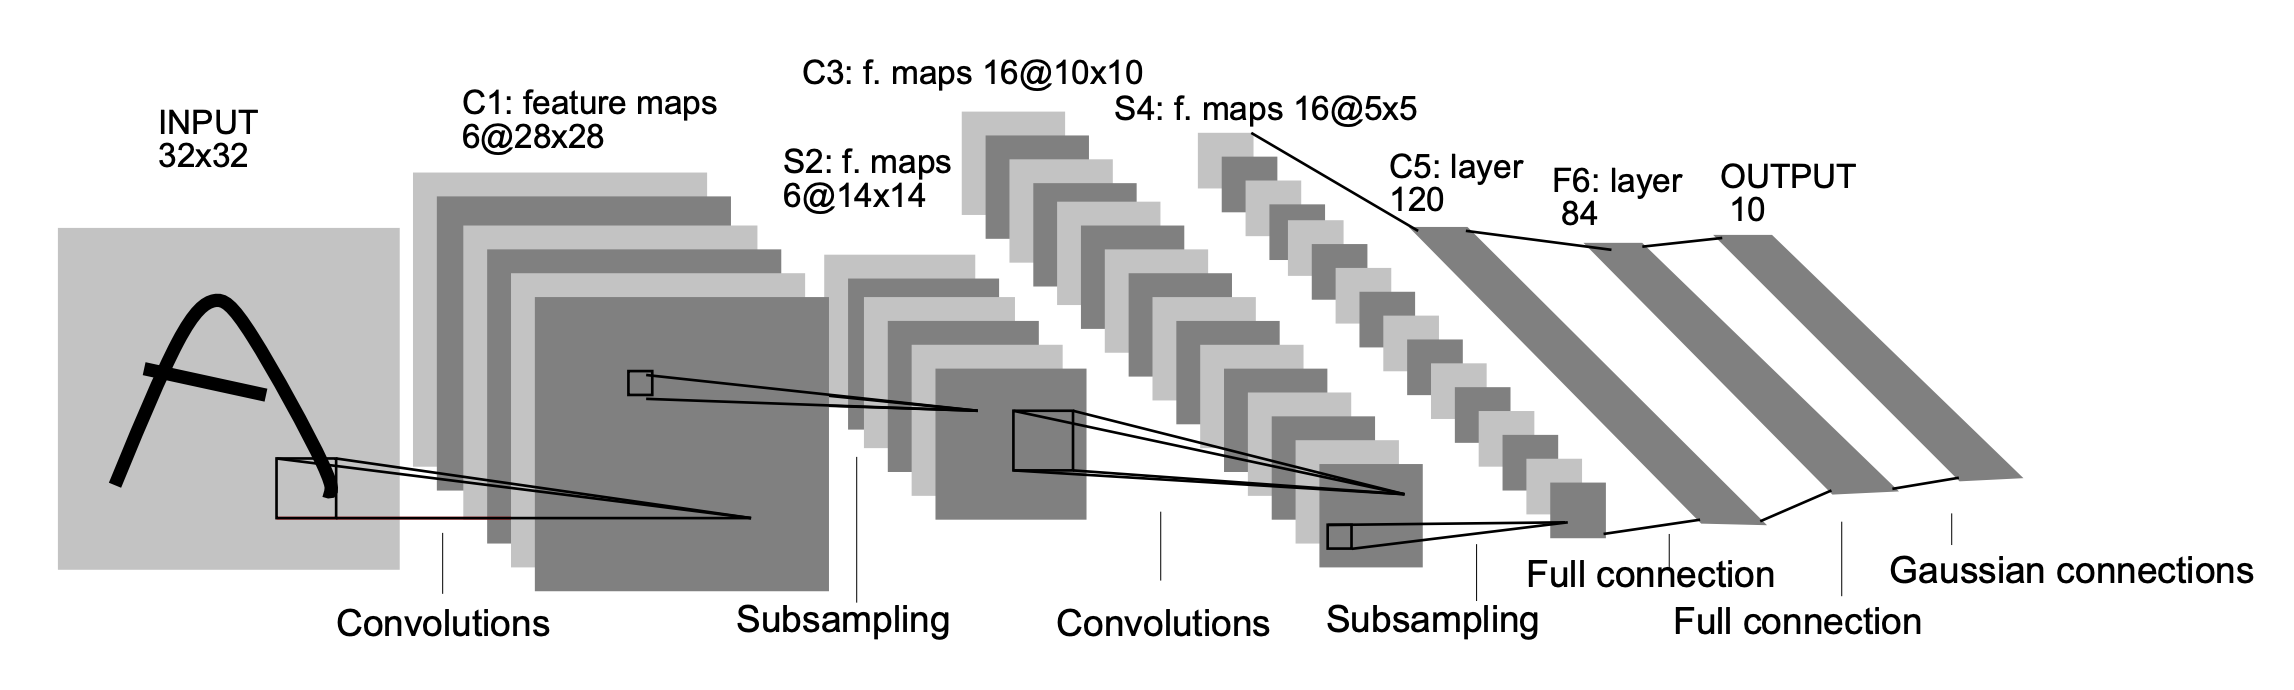
\includegraphics[width=0.5\textwidth]{graphs/LeNet} 
    \caption{Architecture of LeNet-5 by LeCun et al. \cite{LeCun}}
    \label{fig: LeNet}
\end{figure}

% Expected performance - overfitting
Increasing the number of layers in a neural network is often believed to provide a better model, given the higher complexity. However, a model can be easily overfit to the training set if the parameters follow the data too closely.
In order to obtain a more generalised model of the data, cross-validation was selected to perform out-of-sample testing on the dataset.
% TODO: Explain cross-validation

% ========================= Implementation ======================== %
\section{Implementation} \label{s-implement}

% Provide name and use of \textit{external libraries} and explain how \textit{model parameters} were selected.\\

% Preprocessing
The primary image manipulation and pre-processing tasks were performed with the aid of the Open Source Computer Vision (OpenCV) and dlib libraries, which are widely used in image processing. The implemented functions range from colour space transformation to face detection and landmark prediction for the binary classification tasks. 
Mathematical manipulation and analysis as well as file handling were mainly carried out using the NumPy and Pandas software libraries.

% Machine learning
As for the implementation of machine learning algorithms, such as SVM, MLP, and the corresponding tools to carry out cross-validation and obtain the confusion matrix, the Scikit-learn library was employed to mainly carry out binary classification tasks. 
Likewise, Keras was implemented for running neural network algorithms, specifically the Convolutional Neural Networks, enabling fast experimentation on a large dataset.
% Plots and graphs
Finally, the Matplotlib plotting library was included to provide visual outputs on the data, such as learning curves, which outline the validation and test accuracies over a range of training samples, such as that shown in Figure \ref{fig: T1-LC}.
% TODO: Explain the curve..?

\begin{figure} [h] % Learning curve of Task 1: emotion (SVM)
  \centering
    \includegraphics[width=0.5\textwidth]{graphs/T1_SVM_RBF} 
    \caption{Learning curve of emotion recognition}
    \label{fig: T1-LC}
\end{figure}

% Model parameters
Each classification task was performed using various functions and parameters. For instance, the SVM was implemented with different Kernels to find the optimum performance of binary classification, such as linear, polynomial (\code{poly}), radial basis function (\code{rbf}), and sigmoid. A sweep of the penalty parameter $C$ was carried out to observe the effects of parameter variations.
In a similar manner, variations in the number of hidden layers, regularisation parameter alpha, and the solver were applied to achieve the optimum response. The log-loss function of the MLP is optimised using the lbfgs or stochastic gradient descent (\code{sgd}).

% Thorough discussion on the training convergence and stopping criterion (use learning curves graphs).\\

% TODO!!

% ======================= Experimental results ====================== %
\section{Experimental result} \label{s-exp-res}

% Describe and discuss results, compare to other approaches in literature or variations of ML solutions.\\
% Include \textit{accuracy prediction scores on a separate test dataset, provided by the module organisers, but not used during training and validation}.\\

% Face detection
As previously explained, the HOG face detector is expected to provide an accuracy higher than that of the Haar Cascade and lower than that of Deep Learning methods. To observe the trade-offs between the performance and complexity of these models, a comparison of the four was carried out with the same 4,000 training data and 1,000 test data for all detectors. Table \ref{tab: face} lays out a comparative view of each method based on the overall accuracy, the true positive rate (TPR), true negative rate (TNR), false positive rate (FPR), false negative rate (FNR), and the time taken in minutes to train and carry out the predictions.

\begin{table}[htp]
\caption{Comparative measures of face detector scores}
\begin{center}
\renewcommand{\arraystretch}{1.5}
\begin{tabular}{|c|c|c|c|c|c|c|}
\hline
Method & Accuracy & TPR & TNR & FPR & FNR & Time\\ \hline
Haar Cascade & 0.78 & 0.77 & 0.40 & 0.03 & 0.72 & 1.88 \\ \hline
HOG with SVM & 0.97 & 0.97 & 1.00 & 0.00 & 0.33 & 2.79 \\ \hline
SSD (DNN) & 0.99 & 0.98 & 1.00 & 0.00 & 0.14 & 4.55\\ \hline
MMOD (CNN) & 0.98 & 0.98 & 1.00 & 0.00 & 0.18 & 10.85\\ \hline
\end{tabular}
\end{center}
\label{tab: face}
\end{table}%

% Classification: binary
The performance of the binary model classifiers were analysed and compared via the calculation of the model accuracy, recall (true positive rate), specificity (true negative rate), and precision based on its respective confusion matrix. 
% Results table
As shown in table \ref{tab: bin}, the MLP classifier with lbfgs solver was often found to be the optimum solution for the binary tasks, as the number of hidden layers were maintained low to avoid overfitting to the training data. 
% Cross validation
Carrying out rotation estimation on the data showed an instance of overfitting for the MLP classifier, as the overall score obtained from a 10-fold cross-validation on task 2 was measured to be 0.79, whereas the SVM classifier with the RBF kernel provided an accuracy as high as 0.84.

\begin{table}[htp]
\caption{Performance measures of binary classifiers}
\begin{center}
\renewcommand{\arraystretch}{1.5}
\begin{tabular}{|c|c|c|c|c|c|}
\hline
Task & Method & Accuracy & Recall & Specificity & Precision\\ \hline
1 & MLP (lbfgs) & 0.93 & 0.95 & 0.86 & 0.96\\ \hline
2 & MLP (lbfgs) & 0.79 & 0.81 & 0.60 & 0.96\\ \hline
3 & MLP (lbfgs) & 0.86 & 0.81 & 0.88 & 0.66\\ \hline
4& SVM (poly) & 0.98 & 0.98 & 0.97 & 0.96\\ \hline
\end{tabular}
\end{center}
\label{tab: bin}
\end{table}%

% Classification: multiclass
The SVM and MLP classifiers were initially trained on the raw image dataset (with lowered image sizes converted to arrays) to carry out multiclass classification on hair colour for the fifth and final task. The linearised formatted of the feature set resulted in a higher complexity with inadequate test scores. Hence, a CNN with the LeNet architecture was implemented, providing a more acceptable test accuracy, as illustrated in Table \ref{tab: mult}.
% CNN data split x2
The training data of this task was divided in two stages for this task in order to provide sufficient validation data for backpropagation. 

% task 5 accuracy table
\begin{table}[htp]
\caption{Performance measures of multiclass classifiers}
\begin{center}
\renewcommand{\arraystretch}{1.5}
\begin{tabular}{|l|c|c|}
\hline
\hspace{1cm} Method & Accuracy & Time\\ \hline
SVM with Sigmoid Kernel & 0.14 & 1.70\\ \hline
SVM with RBF Kernel & 0.30 & 2.37\\ \hline
MLP with SGD solver & 0.49 & 0.38\\ \hline
MLP with LBFGS solver & 0.60 & 0.20\\ \hline
CNN with LeNet architecture & 0.81 & 7.85\\ \hline
\end{tabular}
\end{center}
\label{tab: mult}
\end{table}%

% CNN test/val plot
As shown in the plot of the training and validation accuracies of the LeNet model throughout the backpropagation process in Figure \ref{fig: CNN}, the model achieved a maximum score of 0.81 after 25 epochs. This is considerably higher than the achieved accuracies of the SVM and MLP model classifiers.

\begin{figure} [h] % LeNet training/test accuracy
  \centering
    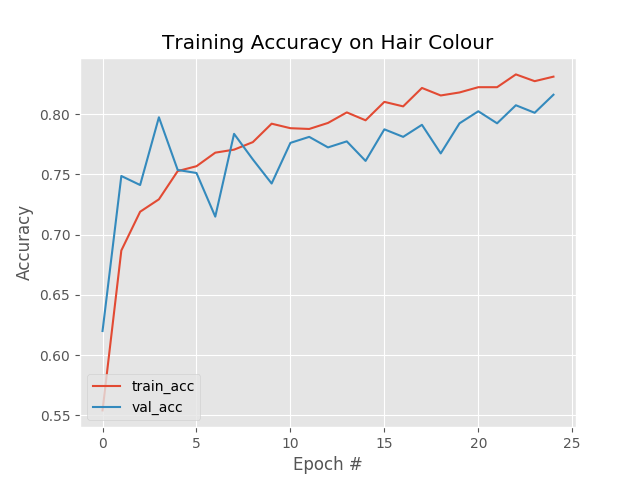
\includegraphics[width=0.5\textwidth]{graphs/T5_CNN_Keras} 
    \caption{LeNet training and validation accuracy variation}
    \label{fig: CNN}
\end{figure}

\break

% ========================== Conclusion ========================== %
\section{Conclusion} \label{s-concl}

% Summaries all findings and suggest direction for future improvement.\\

% General overview
A comparative analysis of several methods of face detection and image classification was carried out on a labelled dataset of 5,000 images using binary and multiclass classifiers with support vector machines and neural networks via OpenCV, dlib, Keras, and Scikit-learn Python libraries for image processing and machine learning. An analysis of the performance and complexity of the models was carried out using cross-validation for a non-biased response and confusion matrices to obtain the statistics of true predictions. 

% binary analysis
The multi-layer perceptron neural network was generally found to provide more accurate binary classification models, except for particular test data on glasses detection (task 3), where the model was overfit. It can therefore be concluded that the higher complexity of neural networks does not necessarily ensure higher prediction scores.

% multiclass analysis
Implementation of the LeNet CNN architecture provided considerably more accurate predictions for the multiclass classification task of hair colour classification. However, higher accuracies can be obtained via the implementation of more advanced convolutional neural networks such as AlexNet, a larger model which includes max pooling, ReLU nonlinearity, and dropout regularisation.

% ========================= Related work ========================== %
\section{Related Work} \label{s-rel-work}

% Summarise latest reserach on the topic, discussing merits/disadvantages of diff approaches.\\

A number of CNN frameworks have been implemented for image classification since the introduction of the LeNet architecture in 1998. Some of the more recent frameworks include GoogLeNet with 19 layers, capable of achieving 6.67\% error with the Inception Module,
and ResNet with 152 layers and an error as low as 3.57\% on the ImageNet dataset \cite{He2006}. The Inception Module in both architectures implements parallel paths of various receptive field dimensions and operations in order to capture sparse correlation patterns, as illustrated in Figure \ref{fig: GoogLeNet}.

\begin{figure} [h] % GoogLeNet Inception Module
  \centering
    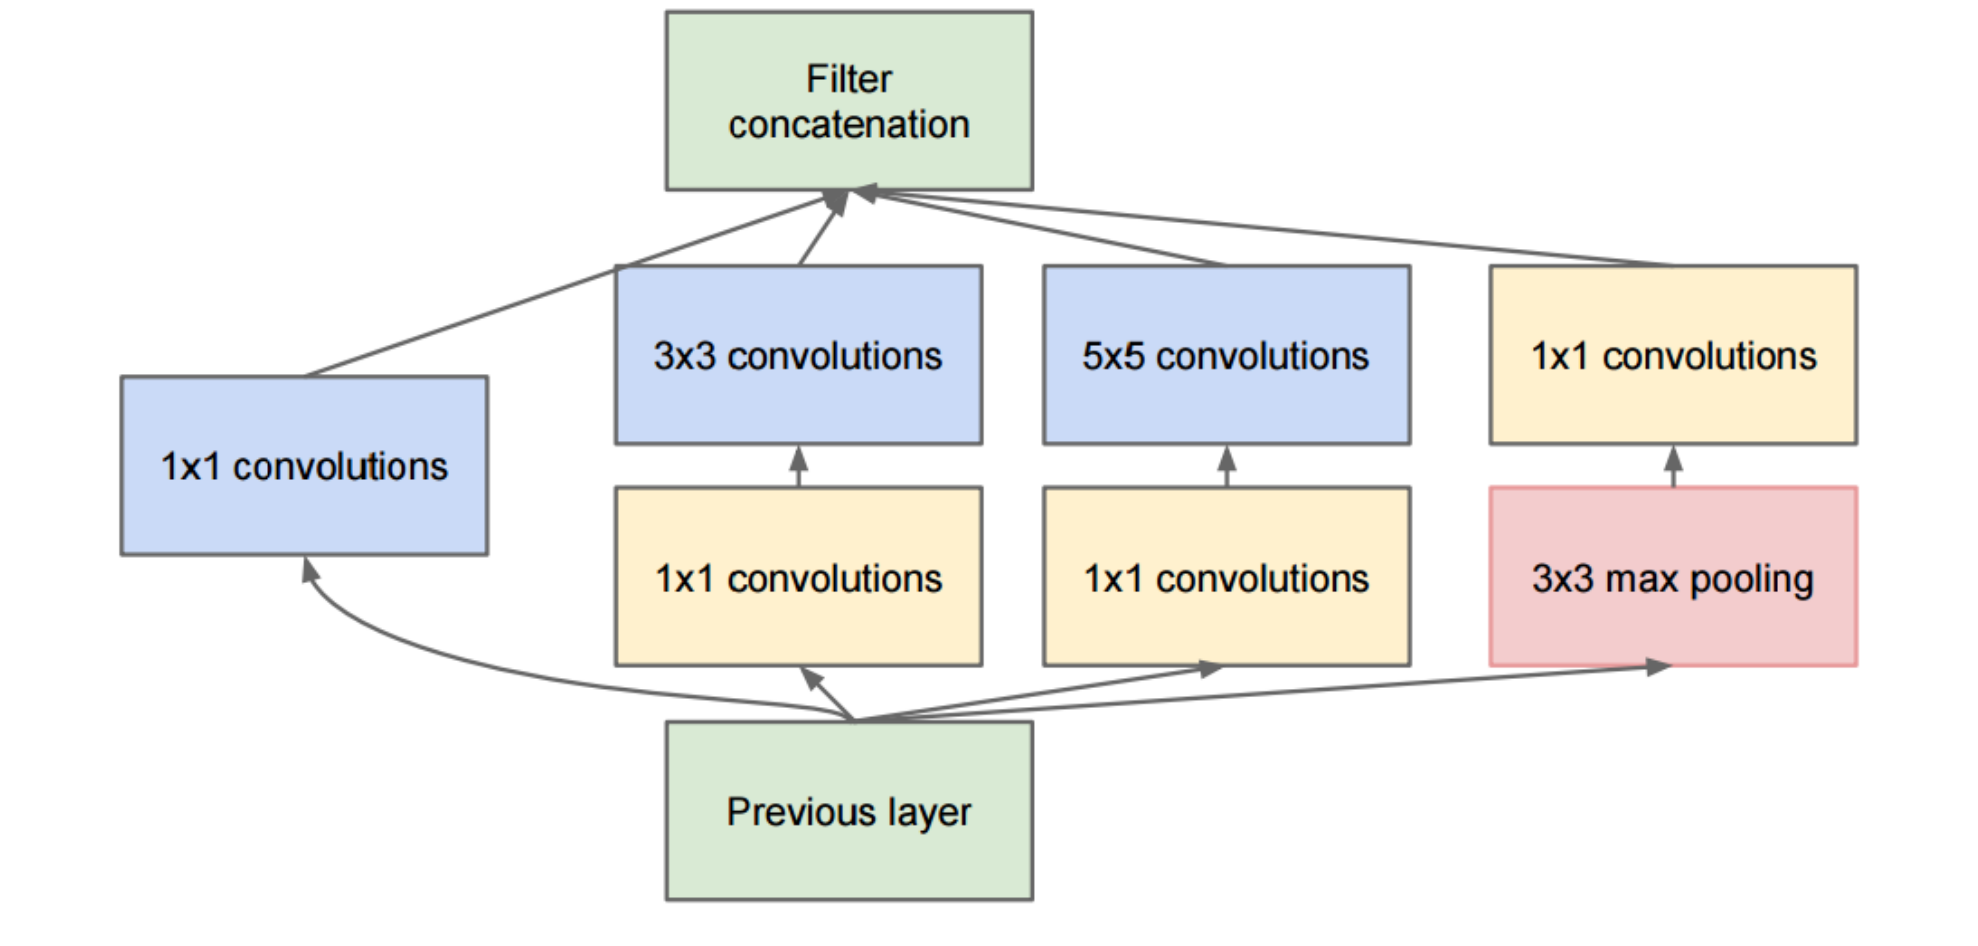
\includegraphics[width=0.5\textwidth]{graphs/GoogLeNet} 
    \caption{Implementation of the Inception Module \cite{Szegedy2015}}
    \label{fig: GoogLeNet}
\end{figure}

Improved variants of the Inception reduces the effects of auxiliary classifiers via the implementation of batch normalisation in order to provide regularised training \cite{Szegedy2015a}. The factorised convolutions and aggressive regularisation of these variants result in more efficient computation in the network.

% ========================== References ========================== %

\bibliographystyle{IEEEtran}
\bibliography{/Users/MaryamH/Documents/BibTex/library}

\end{document}
